\section{Введение}
\subsection{Актуальность работы}
Кровь—это соеденительная ткань внутри организма, она состоит из форменных элементов (эритроцитов, лейкоцитов, тромбоцитов), а так же водного раствора белков и свёртывающих веществ-плазмы. Объёмная доля форменных элементов в общем объеме называется гематокритом и составляет примерно 45\%
\begin{figure}[h]
\centering
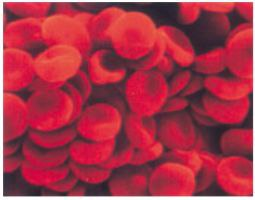
\includegraphics[width=0.3\linewidth]{erotr.jpg}
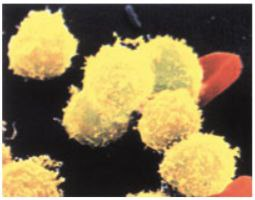
\includegraphics[width=0.3\linewidth]{leiko.jpg}
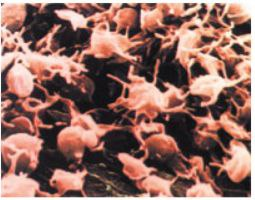
\includegraphics[width=0.3\linewidth]{trombo.jpg}
\caption{ Электронные фотографии элементов крови.1—эритроциты, 2—лейкоциты, 3—тромбоциты. \cite{rls:2003}}
\label{fig:mpr}
\end{figure}\\
Функций у крови несколько: она является транспортным средством, поддерживает постоянство «внутренней среды» организма (гомеостаз), играет главную роль в защите от чужеродных веществ.

С развитием медицины и науки в целом, появилась необходимость в изучении течения крови. Зная как движется кровь в организме, мы получаем более масштабную картину того, как работает наш организм, можем помочь поставить диагноз, спрогнозировать развитие заболеваний, подобрать оптимально лечение.

В изучении течения крови не малую роль играет вычислительная гидродинамика. Её главное достоинство— возможность проводить практически неограниченное число численных экспериментов без опасности для жизни и здоровья испытуемого, в отличие от традиционных методов лечения, где все эксперименты ставятся на органах животных.

\subsection{Общее описание течения крови в организме}
Кровь движется по замкнутой системе сосудов,циркулируя от сердца и обратно. Кровеносная система человека — сложная, разветвленная сеть, состоящая из вен, артерий и капилляров, соединяющих артерии и вены. Кровообращение состоит из двух кругов.

Малый круг начинается в правом желудочке, при сокращении которого венозная кровь попадает в легочный ствол и, протекая через легкие, отдает диоксид углерода и насыщается кислородом. Обогащенная кислородом кровь из легких по легочным венам поступает в левое предсердие, где заканчивается малый круг. Большой круг начинается в левом желудочке, при сокращении которого кровь, обогащенная кислородом, нагнетается в аорту, артерии, артериолы и капилляры всех органов и тканей, а оттуда по венулам и венам притекает в правое предсердие, где и заканчивается большой круг.

Кровь движется по сосудам под воздействием периодических сокращений сердечной мышцы, описываемых сердечным циклом. Под сердечным циклом понимают период, охватывающий одно сокращение и одно расслабление предсердий и желудочков. Общая длительность сердечного цикла при частоте сердечных сокращений 75 уд/мин равна 0,8 с. Систола (0,33с) — фаза сердечного цикла, включающая сокращение миокарда и изгнание крови из сердца в сосудистую систему. Диастола (0,47) — фаза сердечного цикла, включающая расслабление миокарда и наполнение полостей сердца кровью.

Все сосуды в человеческом организме можно условно разделить на аорту(диаметр ~ 15.3 мм), артерии(диаметр ~ 0.5—2.5 мм), полые вены(диаметр ~ 12 мм), вены (диаметр ~ 0.75—2.7 мм) и капилляры(диаметр ~ 8 мкм).

Стенку кровеносного сосуда (за исключением капилляров) условно можно разделить на три слоя: интима – внутренний слой, медиа – средний слой, адвентиция – внешний слой (рис. 2).
В зависимости от состава сосудистой стенки, артерии условно делят на эластичный или мышечный типы . Артерии эластичного типа – сосуды относительно большого диаметра, расположенные ближе к сердцу (например аорта), медиа которых содержит большое количество упругих мембран. Число упругих мембран убывает при уменьшении размера сосуда. Они практически отсутствуют в артериях мышечного типа. Артерии мышечного типа находятся на периферии (например, бедренная артерия). В среднем слое артерий мышечного типа доминируют гладкомышечные клетки. Вены, в отличие от артерий, делятся по размеру внутреннего диаметра. У вен толщина стенок и толщина среднего слоя намного меньше, чем у артерий. При этом у вен толще внешний слой. \cite{Rhodin:1980} 


\begin{figure}[h]
\centering
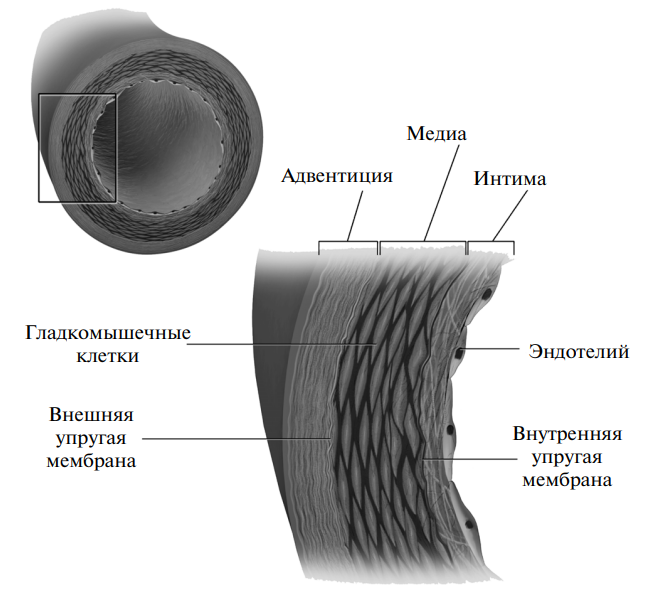
\includegraphics[width=0.3\linewidth]{stenki.png}
\caption{ Типовое строение стенки кровеносного сосуда \cite{blausen:2014}.}
\label{fig:mpr}
\end{figure}

Кровь, двигаясь по сосудам, испытывает сопротивление движению со стороны сосудов и из-за её вязкости. Величина сопротивления зависит от диаметра сосуда, его длины, скорости кровотока. Поэтому сердце выбрасывает кровь в сосудистую систему под большим давлением. В разных отделах сосудистой системы давление крови будет разным. В аорте среднее давление в 100 мм рт.ст. колеблется в диапазоне от 120 мм рт.ст. при систоле до 80 мм рт.ст. при диастоле. Разница между ними—пульсовое давление. По мере движения крови давление в сосудистом русле падает. Таким образом, непрерывные, ритмические сокращения сердца, преодолевая сопротивление, создают и поддерживают разность кровяного давления между артериальным и венозным участком сосудистой системы. Эта разность давлений и является главной причиной движения крови по сосудам из области высокого давления в область более низкого.

При движении крови по сосудам различают линейную и объемную скорость кровотока. Линейная скорость определяется суммарным сечением сосудистой системы. Она максимальна в аорте — до 50 см/сек и минимальна в капиллярах — около нуля. В венозном отделе сосудистой системы линейная скорость вновь возрастает. Линейная скорость в полых венах в два раза меньше, чем в аорте и равна примерно 25 см/мин, поскольку в организме на одну артерию приходится две вены,Объемная скорость кровотока — это количество крови, протекающее через общее сечение сосудистой системы в единицу времени. Она одинакова во всех отделах сосудистой системы. Через любое сечение сосудистой системы в единицу времени всегда проходит одинаковое количество крови.

Состоит кровь, как уже было сказано ранее, из форменных клеток и плазмы. Численную долю объёма крови, приходящуюся на клетки, называют гематокритом. Его значение варьируется в зависимости от пола, возраста в границах 0.37 - 0.54. 99 \% гематокрита приходится на эритроциты. Эритроциты— двояковогнутые диски, размерами 7-8 мкм, их количество так же зависит от параметров организма и варьируется от 3.8 до 5.6 миллионов клеток на 1 мкл, а объём от 73 до 83 $10^{-15}$л. Лейкоциты-ядерные клетки округлой формы, их количество на 1 мкл составляет 4.5–11 тысяч, а размеры 4-20 мкм, количество тромбоцитов 150-400 тысяч на 1 мкл и размеры 2-4 мкм. 60 \% от объёма крови приходится на плазму — жидкое межклеточное вещество, содержащее 90—93 \% воды и 7—10 \% сухого вещества (белки, углеводы, соли).

Вязкость крови обычно оценивают: 4.3-4.9 мПа$\cdot$с, а её плотность 1.052—1.0604 г/см\textsuperscript{3}. В зависимости от наличия заболеваний, определенного образа жизни и питания эти показатели могут отходить от нормы. 

Ламинарное течение – упорядоченный режим течения вязкой жидкости, характеризующийся отсутствием перемешивания между слоями жидкости. Течение жидкости с завихрениями называется турбулентным. 
Наличие условий, при которых ламинарное течение перестает быть устойчивым, зависит от числа Рейнольдса:
$$Re=\frac{V\cdot S\cdot \rho}{\eta}$$
где v – скорость течения жидкости, S– сечение трубы, $\rho$- плотность жидкости, $\eta$- вязкость жидкости.

Для гладких труб Re= 2300. Если Re известно, то становится возможным предсказать, будет ли поток ламинарным или турбулентным. Если для определенного течения число Рейнольдса не превышает некоторого критического значения, то ламинарное течение устойчиво. Если же оно больше, то в потоке жидкости возникают завихрения. Re для крови равно 900-1600. Движение крови в организме, в основном, ламинарное. Однако, при определенных условиях, кровоток может приобретать и турбулентный характер.

Турбулентность проявляется в полостях сердца (велико значение d), в аорте и вблизи клапанов сердца (высокая скорость движения крови). При интенсивной физической нагрузке скорость движения крови увеличивается, и это может вызвать турбулентность в кровотоке. При некоторых патологических процессах, приводящих к аномальному снижению вязкости крови, кровоток в крупных кровеносных сосудах может стать турбулентным.  При наличии атеросклеротических бляшек в просвете сосудов имеются локальные сужения, приводящие к возникновению турбулентности в течении крови. 

\subsection{Вывод}
 С точки зрения гидродинамики кровоток представляет из себя пульсирующее с низкой частотой течение мелкодисперсной суспензии в замкнутой системе каналов кругового сечения с эластичными стенками, осложнённое локальными эффектами ламинарно-турбулентного перехода.
